\begin{minipage}{0.75\linewidth}
\begin{figure}[h]
    \centering
    \begin{adjustbox}{max width=1.0\linewidth, keepaspectratio}
        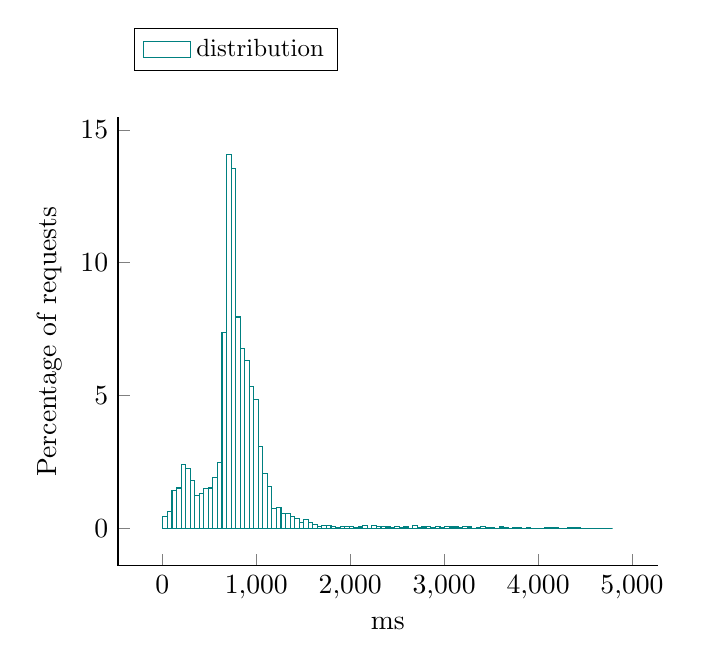
\begin{tikzpicture}
            \begin{axis}[ylabel = Percentage of requests, 
xlabel = ms, 
legend style = {nodes={scale=0.9, transform shape}, at={(0.03,1.2)}, anchor=north west, draw=black, fill=white, align=left, legend columns=3},
area style, mark size = 0pt,
 cycle list name = exotic,
  axis lines* = left]
		\addplot +[ybar interval] coordinates {
			 (6, 0.4375)
			 (54.36, 0.640625)
			 (102.72, 1.42188)
			 (151.08, 1.51562)
			 (199.44, 2.39062)
			 (247.8, 2.26562)
			 (296.16, 1.8125)
			 (344.52, 1.25)
			 (392.88, 1.29688)
			 (441.24, 1.5)
			 (489.6, 1.51562)
			 (537.96, 1.90625)
			 (586.32, 2.46875)
			 (634.68, 7.375)
			 (683.04, 14.0625)
			 (731.4, 13.5469)
			 (779.76, 7.95312)
			 (828.12, 6.76562)
			 (876.48, 6.3125)
			 (924.84, 5.34375)
			 (973.2, 4.85938)
			 (1021.56, 3.09375)
			 (1069.92, 2.04688)
			 (1118.28, 1.5625)
			 (1166.64, 0.75)
			 (1215, 0.765625)
			 (1263.36, 0.546875)
			 (1311.72, 0.5625)
			 (1360.08, 0.4375)
			 (1408.44, 0.359375)
			 (1456.8, 0.21875)
			 (1505.16, 0.328125)
			 (1553.52, 0.234375)
			 (1601.88, 0.15625)
			 (1650.24, 0.078125)
			 (1698.6, 0.109375)
			 (1746.96, 0.09375)
			 (1795.32, 0.078125)
			 (1843.68, 0.03125)
			 (1892.04, 0.0625)
			 (1940.4, 0.0625)
			 (1988.76, 0.078125)
			 (2037.12, 0.03125)
			 (2085.48, 0.046875)
			 (2133.84, 0.109375)
			 (2182.2, 0)
			 (2230.56, 0.09375)
			 (2278.92, 0.0625)
			 (2327.28, 0.0625)
			 (2375.64, 0.046875)
			 (2424, 0.03125)
			 (2472.36, 0.078125)
			 (2520.72, 0.03125)
			 (2569.08, 0.046875)
			 (2617.44, 0)
			 (2665.8, 0.09375)
			 (2714.16, 0.015625)
			 (2762.52, 0.046875)
			 (2810.88, 0.0625)
			 (2859.24, 0.03125)
			 (2907.6, 0.078125)
			 (2955.96, 0.03125)
			 (3004.32, 0.0625)
			 (3052.68, 0.046875)
			 (3101.04, 0.046875)
			 (3149.4, 0.03125)
			 (3197.76, 0.0625)
			 (3246.12, 0.046875)
			 (3294.48, 0)
			 (3342.84, 0.03125)
			 (3391.2, 0.0625)
			 (3439.56, 0.015625)
			 (3487.92, 0.03125)
			 (3536.28, 0)
			 (3584.64, 0.046875)
			 (3633, 0.03125)
			 (3681.36, 0)
			 (3729.72, 0.015625)
			 (3778.08, 0.015625)
			 (3826.44, 0)
			 (3874.8, 0.015625)
			 (3923.16, 0)
			 (3971.52, 0)
			 (4019.88, 0)
			 (4068.24, 0.015625)
			 (4116.6, 0.03125)
			 (4164.96, 0.015625)
			 (4213.32, 0)
			 (4261.68, 0)
			 (4310.04, 0.015625)
			 (4358.4, 0.015625)
			 (4406.76, 0.015625)
			 (4455.12, 0)
			 (4503.48, 0)
			 (4551.84, 0)
			 (4600.2, 0)
			 (4648.56, 0)
			 (4696.92, 0)
			 (4745.28, 0)
			 (4793.64, 0.015625)
		};
\addlegendentry{distribution};
           \end{axis}
      \end{tikzpicture}
  \end{adjustbox}
  \caption{Response time distribution - req = ReadTimeline-3}
\end{figure}
\end{minipage}\hfill\begin{minipage}{0.18\linewidth}
\begin{table}[h]
\begin{tabular}{|cc|}
\hline
\textbf{} & \textbf{ms}\\ \hline
 \Xhline{0.005\arrayrulewidth}
min & 6\\
 \Xhline{0.005\arrayrulewidth}
max & 4842\\
 \Xhline{0.005\arrayrulewidth}
mean & 792\\
 \Xhline{0.005\arrayrulewidth}
std & 403\\
\hline
\hline
 \Xhline{0.005\arrayrulewidth}
25th & 669\\
 \Xhline{0.005\arrayrulewidth}
50th & 758\\
 \Xhline{0.005\arrayrulewidth}
75th & 911\\
 \Xhline{0.005\arrayrulewidth}
80th & 958\\
 \Xhline{0.005\arrayrulewidth}
85th & 1002\\
 \Xhline{0.005\arrayrulewidth}
90th & 1075\\
 \Xhline{0.005\arrayrulewidth}
95th & 1277\\
 \Xhline{0.005\arrayrulewidth}
99th & 2695\\
\hline
\end{tabular}
\caption{Response time}
\end{table}
\end{minipage}\hfill